\documentclass[../Main.tex]{subfiles}

\begin{document}

\begin{tcolorbox}[colback=light-orange, boxrule=0pt]
  \begin{multicols}{3}
    \textcolor{blue}{\textbf{ABSTRACT:}}
Phytoplankton blooms annually occur in spring and fall.
Because of their great ecological impact, phytoplankton blooms are frequently addressed in research.
Blooms are caused by physical forcing that influence stratification and therefore nutrient and light availability.
% Previoulsy, the effects of physical forcing on phytoplankton growth have been studied using satellite images and water samples.
%% Physical parameters have mostly been limited to temperature, light, and density.
% The lack of precision and continuity of collected data often challenges finding correlations.
Previously, identifying physical drivers of pythoplankton blooms has been challenging due to low resolution.
%
Here we show an overview of a new high-resolution dataset measured by gliders in the Baltic Sea from March to October 2021.
The data provide insight into two major phytoplankton blooms that occurred from mid-March to April and from mid-May to early July and one minor bloom after September.
We reveal that the blooms do not depend on the same physical drivers.
The first bloom took place under high wind stress, low temperature and low radiation and the second bloom is driven by warm temperatur, high radiation and low wind stress.
% Phytoplankton blooms are caused by different factors that largely influence the distribution of phytoplankton in water stratification. 
Our results show the possibility to find relationships between different physical drivers of phytoplankton blooms when analyzing high-resolution data.
\ \\
\ \\
    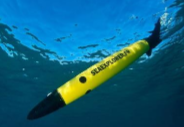
\includegraphics[width=0.33\textwidth]{Glider.png}
 \end{multicols}
\end{tcolorbox}
\end{document}
